% ═══════════════════════════════════════════════════════════════════════
\section{Le triangle et le tapis de Sierpiński}
% ═══════════════════════════════════════════════════════════════════════

\begin{frame}{Figure 3.4 --- Construction par retraits successifs}
  \small $S_0$ : un triangle équilatéral plein de côté $1$. On joint les
  milieux des côtés, on retire (l'intérieur du) triangle central : $S_1$,
  trois triangles de côté $\tfrac12$. On recommence dans chacun.
  \FigBox[0.3\textheight]{%
    \begin{tikzpicture}[scale=2.3]
      \foreach \n in {0,...,4}{
        \begin{scope}[shift={(\n*1.12,0)}]
          \input{figures/fractales/sierpinski-\n.tikz}
          \node[etiq, sectioncolor] at (0.5,-0.13) {$S_{\n}$};
        \end{scope}}
    \end{tikzpicture}}
  \small Le triangle de Sierpiński est $S = \lim_{n\to\infty} S_n$.
  \begin{itemize}
    \item Les $S_n$ sont des points de $\big(\Comp{\R^2},\dH\big)$ :
      $S_n\to S$ veut dire $\dH(S_n,S)\to0$ (définition 2.10).
    \item Comme $S_{n+1}\subseteq S_n$ : $S = S_0\cap S_1\cap S_2\cap\cdots$,
      les points jamais retirés.
  \end{itemize}
\end{frame}

\begin{frame}{Ni aire, ni longueur}
  \small Chaque triangle est remplacé par trois triangles de côté moitié,
  donc d'aire quatre fois plus petite (facteur $k^2$, chapitre 1) :
  \[
    \Aire(S_n) = \left(\frac34\right)^{\!n}\frac{\sqrt3}{4}
    \xrightarrow[n\to\infty]{} 0 .
  \]
  \begin{itemize}
    \item $S$ est contenu dans chaque $S_n$ : son aire est nulle.
    \item Mais $S$ n'est pas vide : il contient les côtés de tous les
      petits triangles, qu'aucune étape ne retire.
    \item Les contours des $3^n$ triangles de $S_n$, tous contenus dans
      $S$, mesurent déjà
      $3^n\cdot3\cdot\big(\tfrac12\big)^n = 3\big(\tfrac32\big)^n\to\infty$.
  \end{itemize}
  \vspace{4pt}
  Ni l'aire ni la longueur ne donnent une mesure finie et non nulle :
  la dimension de similitude (section 5) éclairera cette situation.
\end{frame}

\begin{frame}{Figure 3.5 --- Le tapis de Sierpiński}
  \small Même procédé sur le carré unité : on le partage en neuf carrés
  de côté $\tfrac13$, on retire celui du centre, on recommence dans les
  huit autres.
  \FigBox[0.36\textheight]{%
    \begin{tikzpicture}[scale=2.1]
      \foreach \n in {0,...,4}{
        \begin{scope}[shift={(\n*1.2,0)}]
          \input{figures/fractales/tapis-\n.tikz}
          \node[etiq, sectioncolor] at (0.5,-0.14) {$T_{\n}$};
        \end{scope}}
    \end{tikzpicture}}
  \small $T_n$ : $8^n$ carrés de côté $\big(\tfrac13\big)^n$ ; son aire,
  $\big(\tfrac89\big)^n$, tend vers zéro.
\end{frame}

\begin{frame}{Remarque 3.1 --- L'ensemble de Cantor}
  \begin{Rem}{Remarque 3.1}
    \small Sur $\intff{0}{1}$ : on retire le tiers central ouvert
    $\intoo{\tfrac13}{\tfrac23}$, puis le tiers central de chacun des deux
    segments restants, et ainsi de suite (Cantor, 1883).
    \FigBox[0.18\textheight]{%
      \begin{tikzpicture}[xscale=8, yscale=0.9]
        % Ensemble de Cantor, étapes 0 à 5
% Fichier généré par generer.py : ne pas modifier à la main.
\fill[fractale]
  (0,0) -- (1,0) -- (1,0.1) -- (0,0.1) -- cycle (0,-0.3) -- (0.3333,-0.3) -- (0.3333,-0.2) -- (0,-0.2) -- cycle (0.6667,-0.3) -- (1,-0.3) -- (1,-0.2) -- (0.6667,-0.2) -- cycle (0,-0.6) -- (0.1111,-0.6) -- (0.1111,-0.5) -- (0,-0.5) -- cycle
  (0.2222,-0.6) -- (0.3333,-0.6) -- (0.3333,-0.5) -- (0.2222,-0.5) -- cycle (0.6667,-0.6) -- (0.7778,-0.6) -- (0.7778,-0.5) -- (0.6667,-0.5) -- cycle (0.8889,-0.6) -- (1,-0.6) -- (1,-0.5) -- (0.8889,-0.5) -- cycle (0,-0.9) -- (0.037,-0.9) -- (0.037,-0.8) -- (0,-0.8) -- cycle
  (0.0741,-0.9) -- (0.1111,-0.9) -- (0.1111,-0.8) -- (0.0741,-0.8) -- cycle (0.2222,-0.9) -- (0.2593,-0.9) -- (0.2593,-0.8) -- (0.2222,-0.8) -- cycle (0.2963,-0.9) -- (0.3333,-0.9) -- (0.3333,-0.8) -- (0.2963,-0.8) -- cycle (0.6667,-0.9) -- (0.7037,-0.9) -- (0.7037,-0.8) -- (0.6667,-0.8) -- cycle
  (0.7407,-0.9) -- (0.7778,-0.9) -- (0.7778,-0.8) -- (0.7407,-0.8) -- cycle (0.8889,-0.9) -- (0.9259,-0.9) -- (0.9259,-0.8) -- (0.8889,-0.8) -- cycle (0.963,-0.9) -- (1,-0.9) -- (1,-0.8) -- (0.963,-0.8) -- cycle (0,-1.2) -- (0.0123,-1.2) -- (0.0123,-1.1) -- (0,-1.1) -- cycle
  (0.0247,-1.2) -- (0.037,-1.2) -- (0.037,-1.1) -- (0.0247,-1.1) -- cycle (0.0741,-1.2) -- (0.0864,-1.2) -- (0.0864,-1.1) -- (0.0741,-1.1) -- cycle (0.0988,-1.2) -- (0.1111,-1.2) -- (0.1111,-1.1) -- (0.0988,-1.1) -- cycle (0.2222,-1.2) -- (0.2346,-1.2) -- (0.2346,-1.1) -- (0.2222,-1.1) -- cycle
  (0.2469,-1.2) -- (0.2593,-1.2) -- (0.2593,-1.1) -- (0.2469,-1.1) -- cycle (0.2963,-1.2) -- (0.3086,-1.2) -- (0.3086,-1.1) -- (0.2963,-1.1) -- cycle (0.321,-1.2) -- (0.3333,-1.2) -- (0.3333,-1.1) -- (0.321,-1.1) -- cycle (0.6667,-1.2) -- (0.679,-1.2) -- (0.679,-1.1) -- (0.6667,-1.1) -- cycle
  (0.6914,-1.2) -- (0.7037,-1.2) -- (0.7037,-1.1) -- (0.6914,-1.1) -- cycle (0.7407,-1.2) -- (0.7531,-1.2) -- (0.7531,-1.1) -- (0.7407,-1.1) -- cycle (0.7654,-1.2) -- (0.7778,-1.2) -- (0.7778,-1.1) -- (0.7654,-1.1) -- cycle (0.8889,-1.2) -- (0.9012,-1.2) -- (0.9012,-1.1) -- (0.8889,-1.1) -- cycle
  (0.9136,-1.2) -- (0.9259,-1.2) -- (0.9259,-1.1) -- (0.9136,-1.1) -- cycle (0.963,-1.2) -- (0.9753,-1.2) -- (0.9753,-1.1) -- (0.963,-1.1) -- cycle (0.9877,-1.2) -- (1,-1.2) -- (1,-1.1) -- (0.9877,-1.1) -- cycle (0,-1.5) -- (0.0041,-1.5) -- (0.0041,-1.4) -- (0,-1.4) -- cycle
  (0.0082,-1.5) -- (0.0123,-1.5) -- (0.0123,-1.4) -- (0.0082,-1.4) -- cycle (0.0247,-1.5) -- (0.0288,-1.5) -- (0.0288,-1.4) -- (0.0247,-1.4) -- cycle (0.0329,-1.5) -- (0.037,-1.5) -- (0.037,-1.4) -- (0.0329,-1.4) -- cycle (0.0741,-1.5) -- (0.0782,-1.5) -- (0.0782,-1.4) -- (0.0741,-1.4) -- cycle
  (0.0823,-1.5) -- (0.0864,-1.5) -- (0.0864,-1.4) -- (0.0823,-1.4) -- cycle (0.0988,-1.5) -- (0.1029,-1.5) -- (0.1029,-1.4) -- (0.0988,-1.4) -- cycle (0.107,-1.5) -- (0.1111,-1.5) -- (0.1111,-1.4) -- (0.107,-1.4) -- cycle (0.2222,-1.5) -- (0.2263,-1.5) -- (0.2263,-1.4) -- (0.2222,-1.4) -- cycle
  (0.2305,-1.5) -- (0.2346,-1.5) -- (0.2346,-1.4) -- (0.2305,-1.4) -- cycle (0.2469,-1.5) -- (0.251,-1.5) -- (0.251,-1.4) -- (0.2469,-1.4) -- cycle (0.2551,-1.5) -- (0.2593,-1.5) -- (0.2593,-1.4) -- (0.2551,-1.4) -- cycle (0.2963,-1.5) -- (0.3004,-1.5) -- (0.3004,-1.4) -- (0.2963,-1.4) -- cycle
  (0.3045,-1.5) -- (0.3086,-1.5) -- (0.3086,-1.4) -- (0.3045,-1.4) -- cycle (0.321,-1.5) -- (0.3251,-1.5) -- (0.3251,-1.4) -- (0.321,-1.4) -- cycle (0.3292,-1.5) -- (0.3333,-1.5) -- (0.3333,-1.4) -- (0.3292,-1.4) -- cycle (0.6667,-1.5) -- (0.6708,-1.5) -- (0.6708,-1.4) -- (0.6667,-1.4) -- cycle
  (0.6749,-1.5) -- (0.679,-1.5) -- (0.679,-1.4) -- (0.6749,-1.4) -- cycle (0.6914,-1.5) -- (0.6955,-1.5) -- (0.6955,-1.4) -- (0.6914,-1.4) -- cycle (0.6996,-1.5) -- (0.7037,-1.5) -- (0.7037,-1.4) -- (0.6996,-1.4) -- cycle (0.7407,-1.5) -- (0.7449,-1.5) -- (0.7449,-1.4) -- (0.7407,-1.4) -- cycle
  (0.749,-1.5) -- (0.7531,-1.5) -- (0.7531,-1.4) -- (0.749,-1.4) -- cycle (0.7654,-1.5) -- (0.7695,-1.5) -- (0.7695,-1.4) -- (0.7654,-1.4) -- cycle (0.7737,-1.5) -- (0.7778,-1.5) -- (0.7778,-1.4) -- (0.7737,-1.4) -- cycle (0.8889,-1.5) -- (0.893,-1.5) -- (0.893,-1.4) -- (0.8889,-1.4) -- cycle
  (0.8971,-1.5) -- (0.9012,-1.5) -- (0.9012,-1.4) -- (0.8971,-1.4) -- cycle (0.9136,-1.5) -- (0.9177,-1.5) -- (0.9177,-1.4) -- (0.9136,-1.4) -- cycle (0.9218,-1.5) -- (0.9259,-1.5) -- (0.9259,-1.4) -- (0.9218,-1.4) -- cycle (0.963,-1.5) -- (0.9671,-1.5) -- (0.9671,-1.4) -- (0.963,-1.4) -- cycle
  (0.9712,-1.5) -- (0.9753,-1.5) -- (0.9753,-1.4) -- (0.9712,-1.4) -- cycle (0.9877,-1.5) -- (0.9918,-1.5) -- (0.9918,-1.4) -- (0.9877,-1.4) -- cycle (0.9959,-1.5) -- (1,-1.5) -- (1,-1.4) -- (0.9959,-1.4) -- cycle;

      \end{tikzpicture}}
    \begin{itemize}
      \item Longueur totale nulle : il reste $2^n$ segments de longueur
        $\big(\tfrac13\big)^n$, soit $\big(\tfrac23\big)^n\to0$.
      \item Pourtant « autant » de points que le segment entier : ce sont
        exactement les nombres de $\intff{0}{1}$ qui s'écrivent en
        base $3$ sans le chiffre $1$.
    \end{itemize}
  \end{Rem}
\end{frame}

\begin{frame}{Note historique 3.2 --- Wacław Sierpiński (1882--1969)}
  \footnotesize
  \begin{columns}[T]
    \begin{column}{0.25\textwidth}
      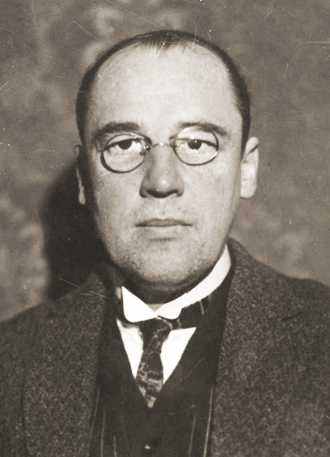
\includegraphics[width=\linewidth]{waclaw-sierpinski.jpg}\\
      {\scriptsize\color{gray}Wacław Sierpiński, en 1928.
      Domaine public, Wikimedia Commons.}
    \end{column}
    \begin{column}{0.72\textwidth}
      \begin{itemize}
        \item Né à Varsovie, alors sous domination russe ; élève de
          Gueorgui Voronoï. Enseigne dans une école secondaire de
          filles, puis doctorat à Cracovie (1906).
        \item À Lwów, en 1909, l'un des tout premiers cours universitaires
          entièrement consacrés à la théorie des ensembles.
        \item Surpris en Russie par la Première Guerre mondiale, interné
          comme ressortissant ennemi (Viatka, puis Moscou), il travaille
          avec Nikolaï Louzine.
        \item C'est là qu'il publie le triangle (1915) et le tapis (1916).
      \end{itemize}
    \end{column}
  \end{columns}
\end{frame}

\begin{frame}{Note historique 3.2 (suite)}
  \small
  \begin{itemize}
    \item Ces constructions servaient la topologie : le triangle est une
      courbe dont chaque point est un point de ramification ; le tapis
      est universel (il contient une copie de toute courbe plane).
    \item 1920 : fonde, avec Stefan Mazurkiewicz, la revue Fundamenta
      Mathematicae, où publiera Banach.
    \item Sous l'occupation, enseigne dans l'université clandestine de
      Varsovie ; perd sa bibliothèque et ses manuscrits dans l'incendie
      de sa maison en 1944.
    \item Plus de $700$ articles, une cinquantaine de livres, et une
      famille d'entiers à son nom : les nombres de Sierpiński.
  \end{itemize}
\end{frame}

\begin{frame}{Pour la classe 3.1 et outil 3.1}
  \begin{Classe}{Les suites géométriques dans les constructions fractales}
    \footnotesize La raison d'une suite prend un sens géométrique :
    longueur multipliée par $\tfrac43$, aire par $\tfrac34$. En
    $4^{\text{e}}$ ou $5^{\text{e}}$ secondaire : construire $K_0$ à $K_3$
    sur du papier pointé isométrique, calculer les longueurs, reconnaître
    une suite géométrique. Une longueur qui croît sans borne dans une
    région bornée : une occasion de parler de limite avant de la définir.
  \end{Classe}
  \begin{Outil}{Construire la courbe de von Koch dans GeoGebra}
    \footnotesize Sur un segment $[AB]$ : points au tiers et aux deux
    tiers, sommet par une rotation de $60^\circ$, quatre segments. Le menu
    Outils $\to$ Créer un nouvel outil en fait un outil (deux points
    $\to$ quatre segments), qu'on applique à chaque segment : $K_2$, puis
    $K_3$. On voit l'idée des SIF --- remplacer chaque segment par une
    copie réduite --- et pourquoi il faut vite un programme : le nombre
    de segments est multiplié par $4$ à chaque étape.
  \end{Outil}
\end{frame}
